\subsection{Deducción de la ecuación de onda}

El movimiento ondulatorio supone la transmisión de una perturbación a través de un punto a otro sin transporte de materia. Nuestro objetivo es encontrar una ecuación matemática que permita conocer el estado de vibración de cada punto a medida que transcurre el tiempo.

\begin{wrapfigure}{r}{0.3\textwidth}
  \centering
  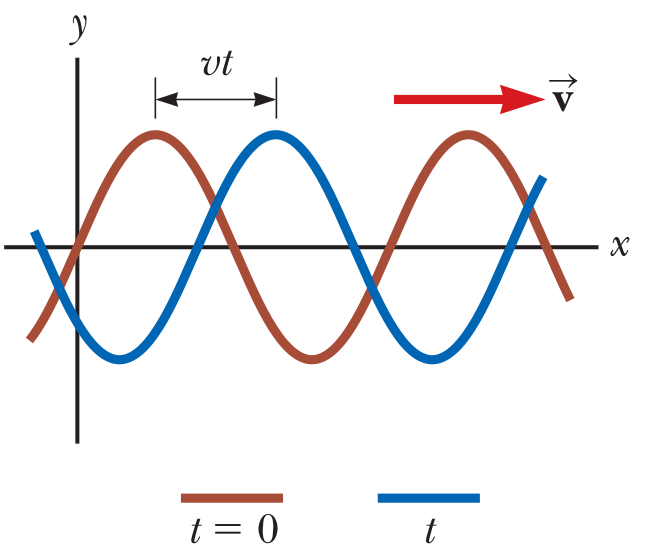
\includegraphics[width=\linewidth]{sin_wave.png}
  \caption{Onda sinusoidal que viaja hacia la derecha con una rapidez \(v\).}
  \label{fig:sin_wave}
\end{wrapfigure}
Para no complicar las cosas, continuemos con el ejemplo de la cuerda. Supongamos que la cuerda tiene un movimiento ondulatorio, y como ya hemos visto, la perturbación en la cuerda crea ondas transversales, y sinusoidales en este caso. 

La onda de color marrón de la figura \ref{fig:sin_wave} describe el estado inicial de la cuerda, es decir, es una instantánea de la onda sinusoidal en \(t=0\). Por otro lado la onda de color azul representa una instantánea de la misma cuerda en algún tiempo posterior \(t\), que llamaremos \(t_1\) para evitar confusión (aunque no se muestra en la figura).

Enfoquemos nuestra atención en un solo pulso de la onda. Si comparamos las instantáneas de la cuerda en \(t=0\) y \(t=t_1\), vemos que el pulso ha viajado una distancia \(v t_1\), donde \(v\) es la velocidad de propagación de la onda. 

Analizando el gráfico vemos que pueden ocurrir dos tipos de movimiento al mismo tiempo:
\begin{itemize}
  \item \textbf{El movimiento de la onda}: ya que la curva marrón, después de que transcurra el tiempo \(t\) llegará a la posición de la curva azul.
  \item \textbf{El movimiento de los elementos del medio}: se mueven de arriba a abajo con un \textit{movimiento armónico simple}. 
\end{itemize}

Si fijamos un tiempo determinado como \(t=0\), como el movimiento que describe la posición de los elementos del medio es un movimiento armónico simple, podemos describir la posición vertical de cada elemento del medio según su posición horizontal con la ecuación:
\begin{equation}
  y(x, t=0) = A \sin(ax)
  \label{eq:sin_wave}
\end{equation}
donde \(A\) es la amplitud, \(a\) es una constante a determinar y \(x\) es la posición horizontal. 

De la ecuación \ref{eq:sin_wave} entonces, se ve que si \(x=0\) entonces \(y=0\), lo que coincide con la figura \ref{fig:sin_wave} en \(t=0\). El siguiente valor de \(x\) para el que \(y\) es cero es \(x=\lambda/2\) como se ve en la figura \ref{fig:sin_wave_2}

Por lo tanto, en base a estas observaciones, podemos escribir:
\[
  y(\lambda/2, t=0) = A \sin(a\lambda/2) = 0
\]
  
\begin{wrapfigure}{l}{0.35\textwidth}
  \centering
  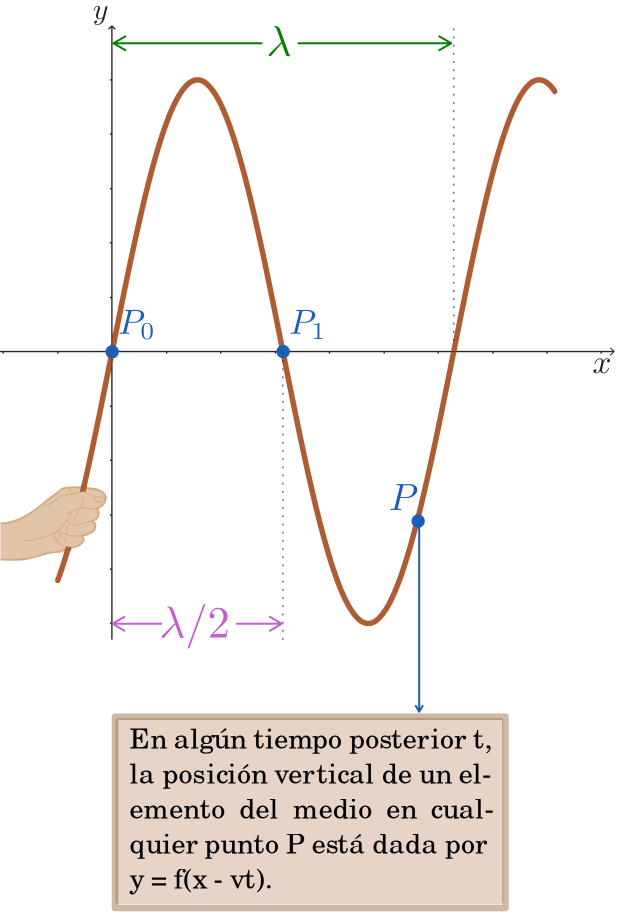
\includegraphics[width=\linewidth]{sin_wave_2.png}
  \caption{Instantánea de la cuerda en \(t=0\) donde una partícula \(P\) cualquiera tiene la misma posición vertical que \(P_0\) cuando la onda viaja una distancia \(v t\).}
  \label{fig:sin_wave_2}
\end{wrapfigure}
Para que esta ecuación sea cierta debe tener \(a\lambda/2 = \pi\) o \(a\lambda/2 = 2\pi\) (en base a la figura \ref{fig:sin_wave_2}), ya que estas posiciones están en fase. En consecuencia, la función que describe las posiciones de todos los elementos del medio a través del que viaja la onda sinusoidal para el instante \(t=0\) se puede escribir como:
\[
  y(x, t=0) = A \sin(\frac{2\pi}{\lambda} x) = 0
\]

Observe que la posición vertical de un elemento del medio es la misma simepre que \(x\) aumente un multiplo entero de \(\lambda\).

Como un pulso de la onda viaja a una velocidad constante \(v\), un elemento cualquiera \(P\) de la cuerda tendrá la misma posición vertical que \(P_0\) en el instante \(t_0\) cuando transcurra un tiempo \(t\) y el pulso de la onda viaje una distancia \(v t\). Entonces, en general podemos expresar la posición de cualquier elemento para todas las posiciones y tiempos como \(f(x - v t)\) donde \(f\) es una función periodica. En este caso \(f\) es la función seno, por lo que resulta:
\[
  y(x, t) = A \sin\left(\frac{2\pi}{\lambda} (x - v t)\right)
\]
  
Sabemos que \(v = \lambda / T ~~ \rightarrow ~~ T = \lambda/v\), por lo que si operamos la ecuación anterior obtenemos:
\begin{align*}
  y(x, t) & = A \sin\left[2\pi \left(\frac{x}{\lambda} - \frac{vt}{\lambda} \right)\right] \\
  y(x, t) & = A \sin\left[2\pi \left(\frac{x}{\lambda} - \frac{t}{T} \right)\right]
\end{align*}

Y recordando las cantidades básicas definidas en la sección \ref{sec:waves_basic_quantities}, podemos escribir:

\begin{equation}
  \boxed{y(x,t) = A \sin(kx - \omega t + \varphi)}
\end{equation}
\begin{itemize}
  \item \(kx\) representa el cambio de fase con la posición (espacial),
  \item \(\omega\) representa el cambio de fase con el tiempo (temporal),
  \item \(\varphi\) es la fase inicial, que determina el estado de oscilación en el origen espacial y temporal.
\end{itemize}